\documentclass[a4paper, 12pt]{article}

\usepackage[table,xcdraw]{xcolor}
\usepackage{enumerate}
\usepackage{graphicx}
\usepackage[T5]{fontenc}
\usepackage[utf8]{inputenc}
\usepackage[margin = 2cm]{geometry}
\usepackage{amsfonts, amsmath, amssymb}
\usepackage[none]{hyphenat}
\usepackage{fancyhdr}
\usepackage{float}
\usepackage{hyperref}
\usepackage{caption}
\usepackage[nottoc, notlot, notlof]{tocbibind}
% \usepackage{rotating}
% \usepackage{tikz}

\captionsetup[table]{skip=5pt}
\pagestyle{fancy}
\fancyhead[L]{Trường Đại học Khoa học Tự nhiên - ĐHQG TP.HCM}
\fancyhead[R]{Nhóm Just $4^{th}$}

\begin{document}
    \begin{titlepage}
        \begin{center}
            % \begin{table}[htbp]
            %     \begin{center}
            %     \begin{tabular}{cc}
            %         \includegraphics[scale = 1]{images/Picture1.png} & \begin{tabular}[c]{@{}l@{}}Đại học Quốc gia TP.HCM\\ Trường Đại học Khoa học Tự nhiên\end{tabular}
            %     \end{tabular}
            %     \end{center}
            % \end{table}

            \vspace*{1cm}
            \Large\textbf{Đại học Quốc gia TP. HCM\\Trường Đại học Khoa học Tự nhiên}\\

            \vfill
            \line(1,0){450}\\[4mm]
            \LARGE\textbf{\MakeUppercase{Báo cáo Lab 01\\ Mỗi quan hệ trong dữ liệu}}\\[3mm]
            \Large{Trực quan hoá dữ liệu (CSC10108)}\\[3mm]
            \Large{Nhóm 17}
            \line(1,0){430}\\
            \vfill

            \vfill
            TP Hồ Chí Minh, ngày 29/04/2021
        \end{center}
    \end{titlepage}

    \tableofcontents
    \thispagestyle{empty}
    \clearpage

    \section{Thông tin nhóm}
    \begin{enumerate}
        \item \textbf{Đường link GitHub}: \url{https://github.com/baolongnguyenmac/CinemaManagementSystem}
        \item \textbf{Danh sách thành viên}
        \begin{table}[H]
            \begin{tabular}{|c|c|l|c|c|}
            \hline
            STT & MSSV     & \multicolumn{1}{c|}{Họ tên} & Email                         & SĐT        \\ \hline
            1   & 18120078 & Ngô Phù Hữu Đại Sơn         & 18120078@student.hcmus.edu.vn & 0919070940 \\ \hline
            2   & 18120201 & Nguyễn Bảo Long             & 18120201@student.hcmus.edu.vn & 0981850699 \\ \hline
            3   & 18120227 & Phạm Văn Minh Phương             & 18120227@student.hcmus.edu.vn & 0981850699 \\ \hline
            4   & 18120253 & Mai Ngọc Tú             & 18120253@student.hcmus.edu.vn & 0981850699 \\ \hline
            5   & 1712424 & Hàn Văn Gia Hiên            & 1712424@student.hcmus.edu.vn & 0911572108 \\ \hline
            \end{tabular}
            \caption{Bảng danh sách thành viên nhóm}
        \end{table}
    \end{enumerate}
    \clearpage

    \section{Phân tích hoàn thiện yêu cầu}

    \subsection{Tổng quan mức độ hoàn thành mỗi yêu cầu}

    \begin{table}[H]
        \begin{tabular}{|c|l|l|c|}
        \hline
        STT & \multicolumn{1}{c|}{Yêu cầu} & \multicolumn{1}{c|}{Công việc}                                                & Hoàn thành (\%) \\ \hline
        1 & Thu thập dữ liệu      & \begin{tabular}[c]{@{}l@{}}- Cài đặt chương trình thu thập dữ liệu\\ - Tiền xử lý dữ liệu\end{tabular}              & 100/100\\ \hline
        2 & Trực quan mối quan hệ & \begin{tabular}[c]{@{}l@{}}- Chọn trường dữ liệu cần trực quan\\ - Trực quan mối quan hệ, giải thích ý nghĩa, \\nhận xét biểu đồ\end{tabular}                          & 90/100 \\ \hline\end{tabular}
        \caption{Bảng phân tích đóng góp cá nhân}
    \end{table}

    \subsection{Mức độ hoàn thành của thành viên nhóm}

    \begin{table}[H]
        \begin{tabular}{|c|l|l|c|}
        \hline
        STT & \multicolumn{1}{c|}{Họ tên} & \multicolumn{1}{c|}{Công việc tham gia}                                                & Hoàn thành (\%) \\ \hline
        1 & Ngô Phù Hữu Đại Sơn      & \begin{tabular}[c]{@{}l@{}}- Thu thập dữ liệu\\- Hồi quy tuyến tính cho cá quan hệ\\ - Biểu diễn quan hệ 2 biến \& 4 biến\end{tabular}              & 20\% \\ \hline
        2 & Nguyễn Bảo Long & \begin{tabular}[c]{@{}l@{}}- Biểu diễn quan hệ 3 biến \& 4 biến\\ - Giải thích lý do sử dụng biểu đồ đường\\ - Nhận xét dữ liệu 3 biến \& 4 biến\end{tabular}                          & 20\% \\ \hline
        5 & Phạm Văn Minh Phương        & \begin{tabular}[c]{@{}l@{}}- Giải thích biểu đồ stacked bar chart\\ - Nhận xét dữ liệu stacked bar chart\end{tabular} & 20\% \\ \hline
        5 & Mai Ngọc Tú       & \begin{tabular}[c]{@{}l@{}}- Giải thích biểu đồ scatter\\ - Nhận xét quan hệ dữ liệu 2 biến\end{tabular} & 20\% \\ \hline
        5 & Hàn Văn Gia Hiên       & \begin{tabular}[c]{@{}l@{}}- \end{tabular} & 20\% \\ \hline
        \end{tabular}
        \caption{Bảng phân tích đóng góp cá nhân}
    \end{table}
    \clearpage

    \section{Thu thập dữ liệu}

    \subsection{Thu thập số liệu thống kê từng ngày}

    \begin{itemize}
        \item Nguồn dữ liệu: \url{https://www.worldometers.info/coronavirus/}
    \end{itemize}

    \subsection{Tiền xử lý}

    \begin{itemize}
        \item Vấn đề dữ liệu gặp phải:
        \item Hướng tiền xử lý:
    \end{itemize}

    \subsection{Khám phá dữ liệu}
    \clearpage 

    \section{Trực quan hoá mối quan hệ giữa các trường dữ liệu}

    \subsection{Chọn trường dữ liệu}

    \begin{itemize}
        \item Với mỗi biến X, Y của tập dữ liệu, ta tính hệ số tương quan 
        $$\rho(X, Y) = \frac{Cov(X, Y)}{\sqrt{Var(X)\times Var(Y)}} = \frac{Cov(X, Y)}{\sigma(X)\times \sigma(Y)}$$
        Với $Cov(X,Y) = E[XY] - E[X]E[Y]$

        \item Từ đó, tính được ma trận hệ số tương quan giữa các cặp biến X, Y trong tập dữ liệu. Biểu diễn ma trận này bằng biểu đồ heatmap để xác định các trường dữ liệu trực quan.
        \begin{figure}[H]
            \begin{center}
                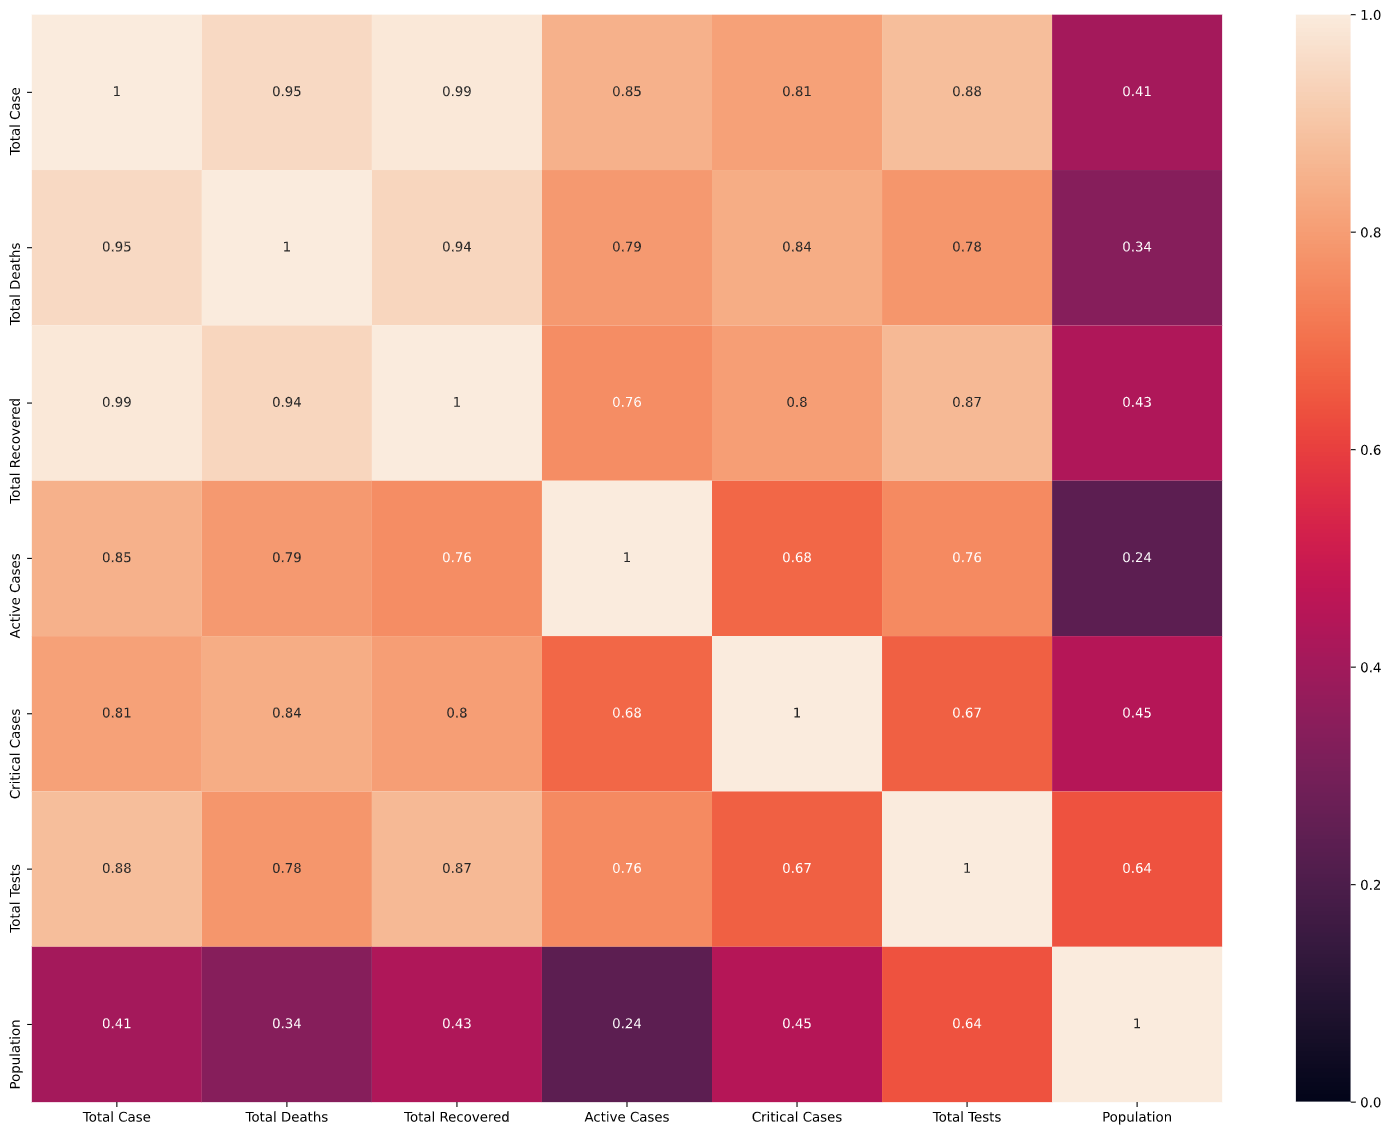
\includegraphics[scale = 0.3]{img/heatmap.png}
                \caption{Biểu đồ thể hiện hệ số tương quan giữa các trường dữ liệu}
            \end{center}
        \end{figure}

        \item Từ biểu đồ trên, chọn ra các cặp thuộc tính có hệ số tương quan lớn hơn 0.7, ta được bảng các cặp thuộc tính sau
        \begin{table}[H]
            \begin{center}
                \begin{tabular}{|c|c|c|c|}
                \hline
                \textbf{STT} & \textbf{Var1} & \textbf{Var2} & \textbf{Hệ số tương quan} \\ \hline
                1    &  Total Deaths     &  Total Cases    & 0.95                 \\ \hline
                2    &  Total Recovered  & Total Cases     & 0.99                 \\ \hline
                3    &  Total Recovered  & Total Deaths    & 0.94                 \\ \hline
                4    &  Active Cases     & Total Cases     & 0.85                 \\ \hline
                5    &  Active Cases     & Total Deaths    & 0.79                 \\ \hline
                6    &  Active Cases     & Total Recovered & 0.76                 \\ \hline
                7    &  Critical Cases   & Total Cases     & 0.81                 \\ \hline
                8    &  Critical Cases   & Total Deaths    & 0.84                 \\ \hline
                9    &  Critical Cases   & Total Recovered & 0.8                 \\ \hline
                10   &  Total Test       & Total Cases     & 0.88                 \\ \hline
                11   &  Total Test       & Total Deaths    & 0.78                 \\ \hline
                12   &  Total Test       & Total Recovered & 0.87                 \\ \hline
                13   &  Total Test       & Active Cases    & 0.76                 \\ \hline
                \end{tabular}
                \caption{Bảng các thuộc tính có hệ số tương quan trên 0.7}
            \end{center}
        \end{table}

        \item Từ bảng trên, ta thấy có 6 thuộc tính có mức độ tương quan với nhau cao là \textbf{Total Case, Total Deaths, Total Recovered, Active Cases, Critical Cases, Total Tests}. Do đó, ta tập trung vào tìm hiểu mối quan hệ giữa các thuộc tính này.
    \end{itemize}

    \subsection{Biểu diễn quan hệ giữa 2 trường dữ liệu}

    \begin{itemize}
        \item Với mỗi 2 trường dữ liệu X, Y trong danh sách các trường dữ liệu xuất hiện trong Table 4, trực quan các điểm dữ liệu thuộc 2 trường đó bằng biểu đồ scatter.
        \item Tiếp đó, tìm một quy luật xấp xỉ phù hợp nhất với dữ liệu quan sát bằng một đường thẳng $\bar{y} = w_0 + xw_1$ với $w_0, w_1$ được tính theo công thức sau
        $$w_1 = \frac{\overline{XY} - \overline{X}.\overline{Y}}{\overline{X^2}-\overline{X}^2}$$
        $$w_0 = \overline{Y} - w_1\overline{X}$$

        \item Lý do sử dụng biểu đồ scatter kết hợp biểu diễn quy luật bằng một đường tuyến tính: Sử dụng biểu đồ scatter để trực quan giúp người đọc dễ dàng nhận ra một sự xấp xỉ tuyến tính (nếu có) tồn tại giữa 2 biến dữ liệu. Cộng thêm việc biểu diễn quy luật bằng một đường tuyến tính, người đọc có thể thấy rõ được "chất lượng" của đường tuyến tính này trong việc giải thích mối quan hệ giữa 2 trường dữ liệu.

        \item Kết quả thu được $C_6^2 = 15$  biểu đồ như sau
        \begin{figure}[H]
            \begin{center}
                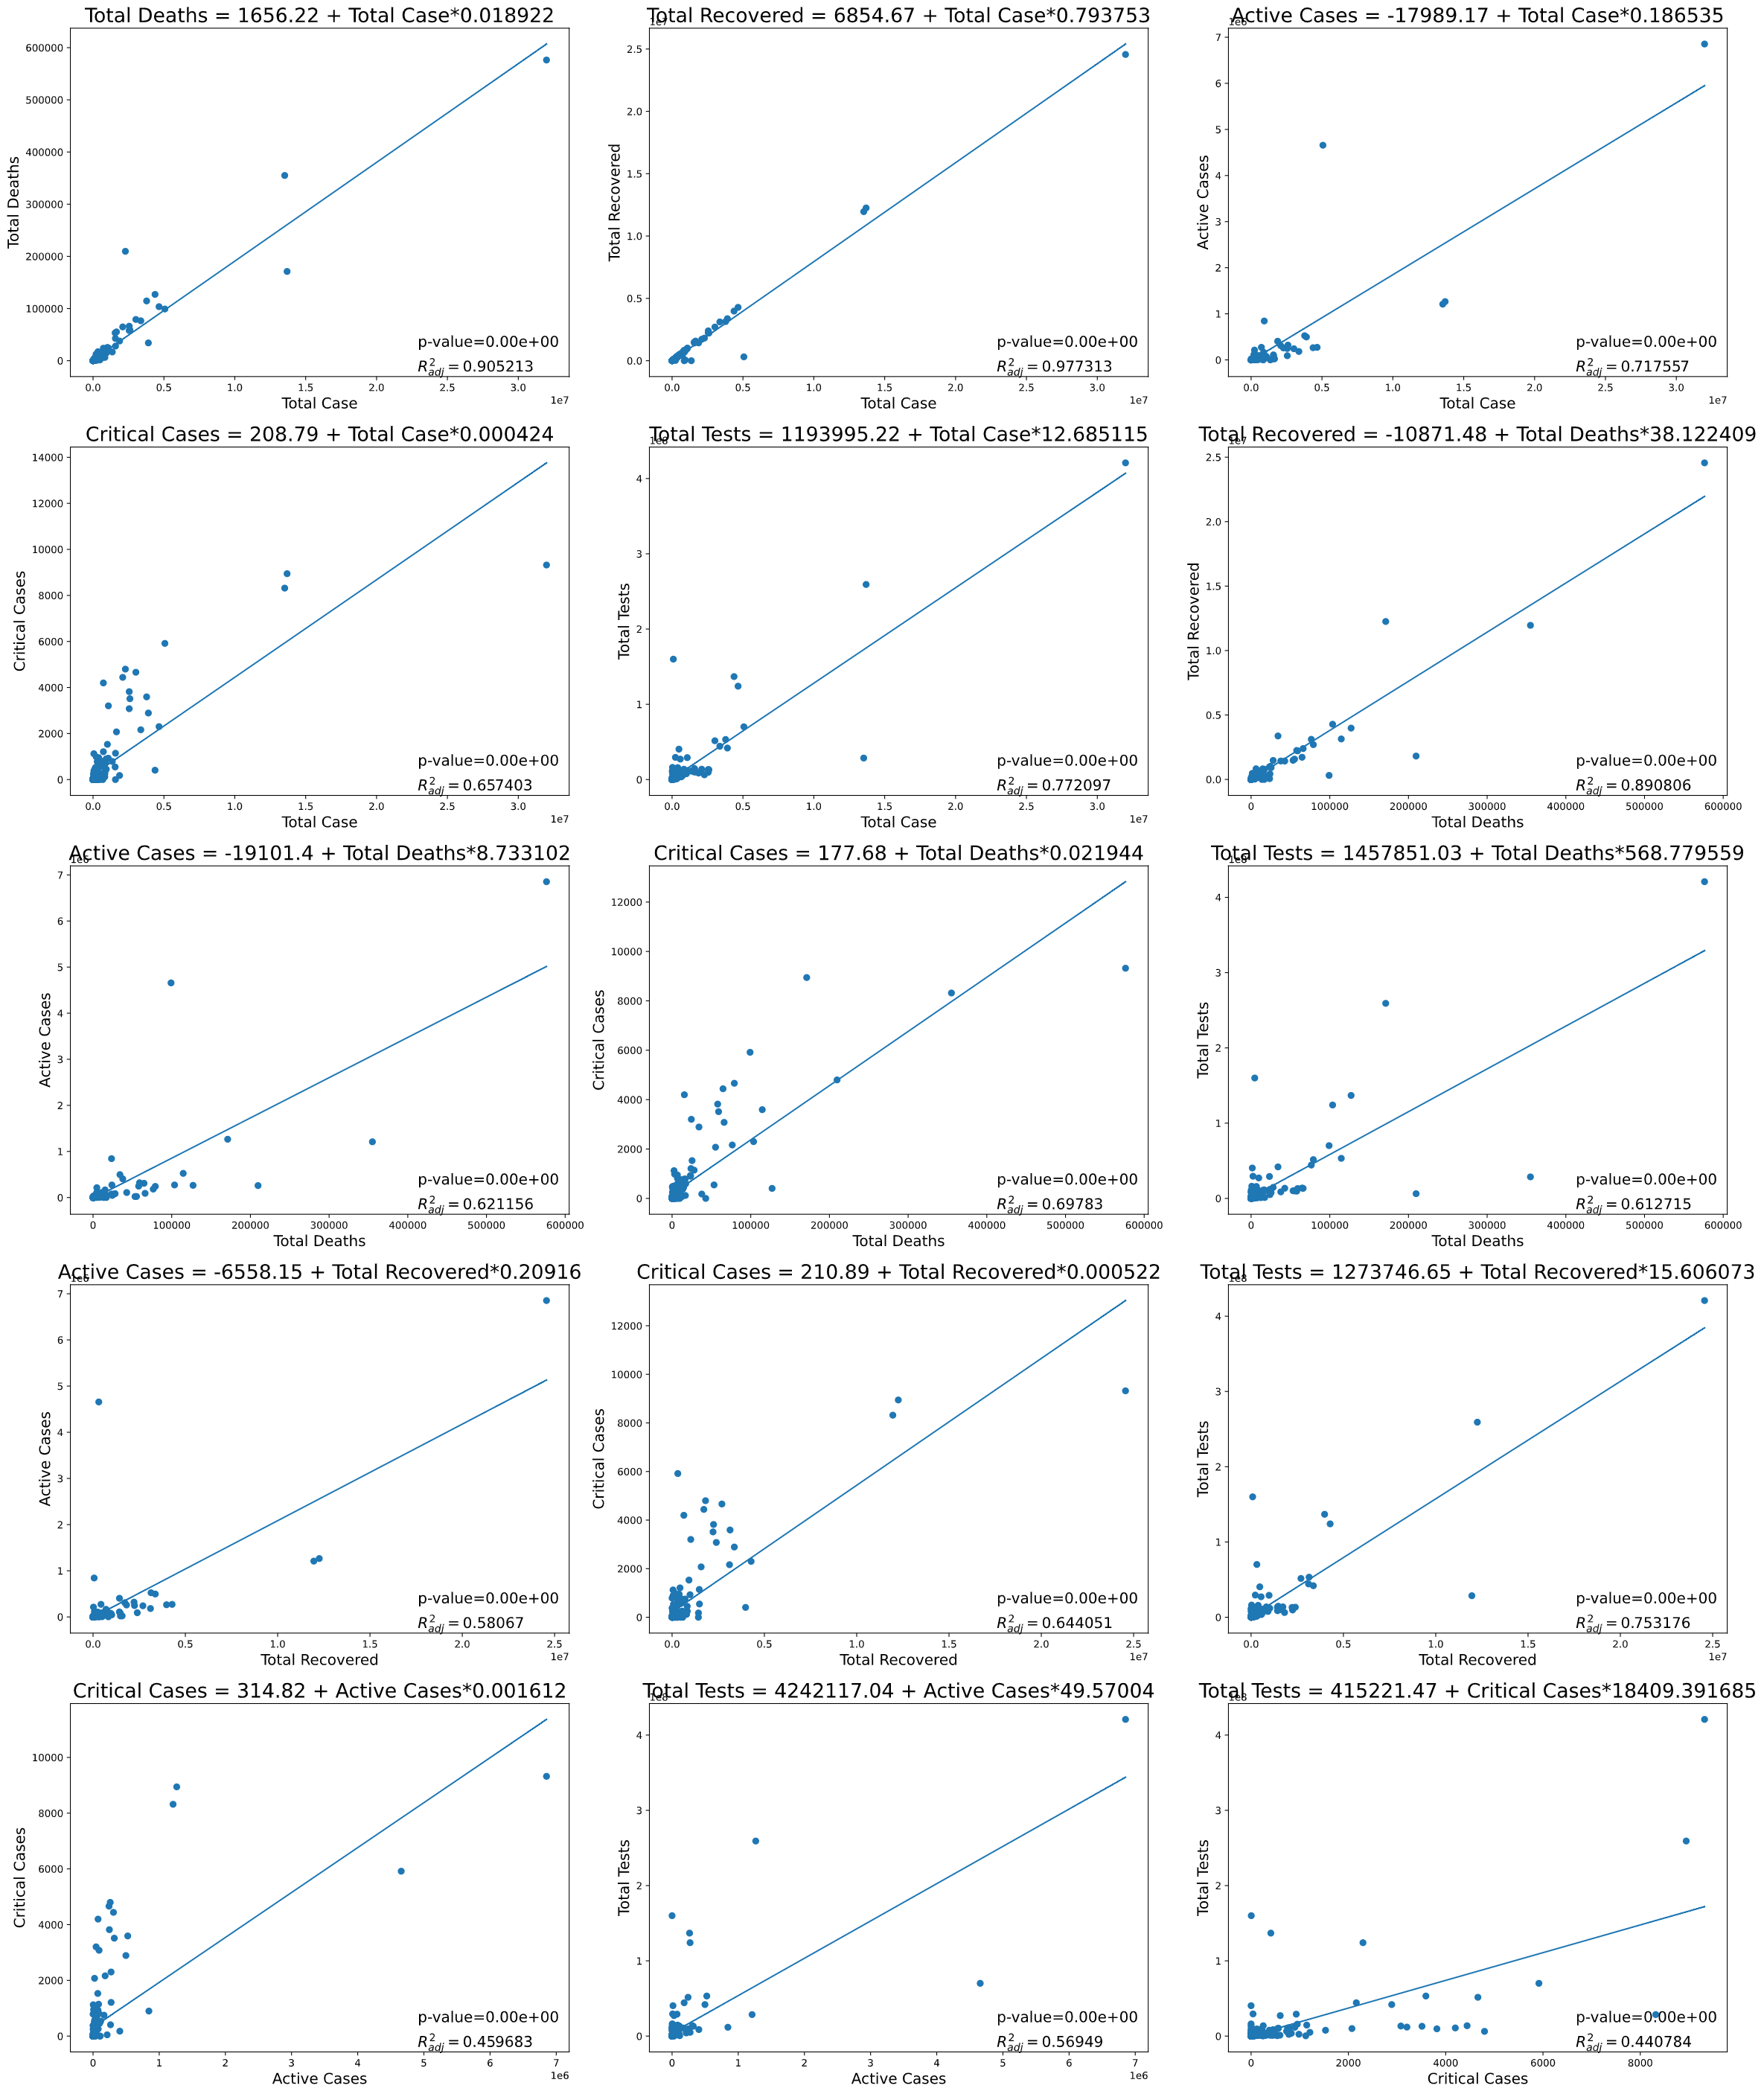
\includegraphics[scale=0.2]{img/scatter.png}
                \caption{Biểu đồ thể hiện mỗi quan hệ giữa 2 biến dữ liệu}
            \end{center}
        \end{figure}

        \item Nhận xét dữ liệu
        \begin{itemize}
            \item Với 5 cặp biến (Độc lập - Phụ thuộc) là \textbf{(Total Case, Total Deaths), (Total Case, Total Recovered), (Total Case, Total Tests), (Total Deaths, Total Recovered), (Total Recovered, Total Tests)}, ta có các kết luận sau
            \begin{itemize}
                \item Chỉ số p-value của các cặp biến này rất nhỏ (trong khoảng [$10^{-180}, 10^{-68}$]). Do đó, các biến độc lập nêu trên có ý nghĩa về mặt thống kê.
                \item Mô hình phù hợp tốt với dữ liệu quan sát về mặt thống kê (p-value trong khoảng [$10^{-180}, 10^{-68}$]).
                \item Hệ số xác định hiệu chỉnh $R_{adj}^2$ của mỗi bộ dữ liệu đều nằm trong khoảng $[75\%, 98\%]$. Do đó, các biến độc lập giải thích được từ 75\% đến 98\% sự thay đổi của các biến phụ thuộc.
                \item Cụ thể phương trình hồi của các cặp biến được ghi trên biểu đồ.
            \end{itemize}

            \item Với các cặp biến còn lại, chỉ số $R_{adj}^2 < 75\%$. Do đó, việc giải thích sự thay đổi của biến phụ thuộc dựa trên biến độc lập là không đủ tin cậy.
            % \item \textbf{(Total Case, Total Deaths)}
            % \begin{itemize}
            %     \item Biến Total Case có ý nghĩa đối với mô hình về mặt thống kê (p-value = 3.27e-113) 
            %     \item Mô hình phù hợp tốt với dữ liệu quan sát về mặt thống kê (p-value = 3.27e-113) 
            %     \item Biến Total Case có thể giải thích được 90.52\% sự thay đổi của biến Total Deaths 
            %     \item Phương trình hồi quy: $Total Deaths = 1656.22 + Total Case \times 0.018922$ 
            % \end{itemize}

            % \item \textbf{(Total Case, Total Recovered)}
            % \begin{itemize}
            %     \item Biến Total Case có ý nghĩa đối với mô hình về mặt thống kê (p-value = 7.72e-72)
            %     \item Mô hình phù hợp tốt với dữ liệu quan sát về mặt thống kê (p-value = 7.72e-72)
            %     \item Biến Total Case có thể giải thích được 77.20\% sự thay đổi của biến Total Tests
            %     \item Phương trình hồi quy: $Total Recovered = 6854.67 + Total Case \times 0.793753$
            % \end{itemize}

            % \item \textbf{(Total Case, Total Tests)}
            % \begin{itemize}
            %     \item Biến Total Case có ý nghĩa đối với mô hình về mặt thống kê (p-value = 7.72e-72)
            %     \item Mô hình phù hợp tốt với dữ liệu quan sát về mặt thống kê (p-value = 7.72e-72)
            %     \item Biến Total Case có thể giải thích được 77.20\% sự thay đổi của biến Total Tests
            %     \item Phương trình hồi quy: $Total Tests = 1193995.22 + Total Case \times 12.685115$
            % \end{itemize}

            % \item \textbf{(Total Deaths, Total Recovered)}
            % \begin{itemize}
            %     \item Biến Total Deaths có ý nghĩa đối với mô hình về mặt thống kê (p-value = 1.53e-106)
            %     \item Mô hình phù hợp tốt với dữ liệu quan sát về mặt thống kê (p-value = 1.53e-106)
            %     \item Biến Total Deaths có thể giải thích được 89.08\% sự thay đổi của biến Total Recovered
            %     \item Phương trình hồi quy: $Total Recovered = -10871.48 + Total Deaths \times 38.122409$
            % \end{itemize}

            % \item \textbf{(Total Recovered, Total Tests)}
            % \begin{itemize}
            %     \item Biến Total Recovered có ý nghĩa đối với mô hình về mặt thống kê (p-value = 4.48e-68)
            %     \item Mô hình phù hợp tốt với dữ liệu quan sát về mặt thống kê (p-value = 4.48e-68)
            %     \item Biến Total Recovered có thể giải thích được 75.31\% sự thay đổi của biến Total Tests
            %     \item Phương trình hồi quy: $Total Tests = 1273746.65 + Total Recovered \times 15.606073$
            % \end{itemize}

            % \item \textbf{(Total Case, Active Cases)}: Biến Total Case không đủ độ tin cậy để giải thích sự thay đổi của biến Active Case (71.75\% < 75\%)
            % \item \textbf{(Total Case, Critical Cases)}: Biến Total Case không đủ độ tin cậy để giải thích sự thay đổi của biến Critical Cases (65.74\% < 75\%)
            % \item \textbf{(Total Deaths, Active Cases)}: Biến Total Deaths không đủ độ tin cậy để giải thích sự thay đổi của biến Active Cases (62.11\% < 75\%)
            % \item \textbf{(Total Deaths, Critical Cases)}: 
            % \item \textbf{(Total Deaths, Total Tests)}: 
            % \item \textbf{(Total Recovered, Active Cases)}: 
            % \item \textbf{(Total Recovered, Critical Cases)}: 
            % \item \textbf{(Active Cases, Critical Cases)}: 
            % \item \textbf{(Active Cases, Total Tests)}: 
            % \item \textbf{(Critical Cases, Total Tests)}: 
        \end{itemize}
    \end{itemize}

    \subsection{Biểu diễn quan hệ giữa 3 trường dữ liệu}

    \subsection{Biểu diễn quan hệ giữa 4 trường dữ liệu}

\end{document}
